\usetikzlibrary{decorations.pathreplacing}
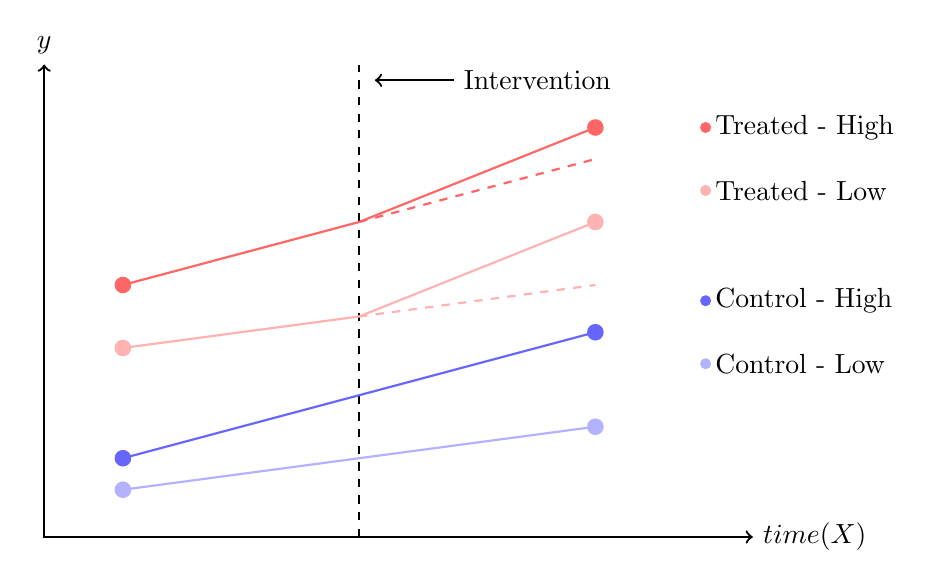
\begin{tikzpicture}[scale=2]
    
	% Draw axes
  \draw [<->,thick] (0,3) node (yaxis) [above] {$y$} |- (4.5,0) node (xaxis) [right] {$time (X)$};
	\draw[thick, color=black, dashed] (2,0) coordinate (t0_0) -- (2,3) coordinate (t0_1);
	
	% Legend
	\coordinate (TH) at (4.2,2.6);
    \fill[red!60] (TH) circle (1pt) node[right, color=black] {Treated - High};
    \coordinate (TL) at (4.2,2.2);
    \fill[red!30] (TL) circle (1pt) node[right, color=black] {Treated - Low};
	\coordinate (CH) at (4.2,1.5);
    \fill[blue!60] (CH) circle (1pt) node[right, color=black] {Control - High};
    \coordinate (CL) at (4.2,1.1);
    \fill[blue!30] (CL) circle (1pt) node[right, color=black] {Control - Low};
	
	% Intervention line
	\draw[thick, -> ] (2.6,2.9) coordinate (t0_0) node[right] {Intervention} -- (2.1,2.9) coordinate (t0_1);

	% Data points
    % control-low
	\draw[thick, color=blue!30] (0.5,0.3) coordinate (c0_0) -- (3.5,0.7) coordinate (c0_1);
    \fill[blue!30] (c0_0) circle (1.5pt);
    \fill[blue!30] (c0_1) circle (1.5pt);
    % control-high
    \draw[thick, color=blue!60] (0.5,0.5) coordinate (c0_0) -- (3.5,1.3) coordinate (c0_1);
    \fill[blue!60] (c0_0) circle (1.5pt);
    \fill[blue!60] (c0_1) circle (1.5pt);
    
    % treated-low
	\draw[thick, color=red!30] (0.5,1.2) coordinate (t0_0) -- (2.0,1.4) coordinate (t0_1);
	\draw[thick, color=red!30] (2.0,1.4) coordinate (t1_0) -- (3.5,2.0) coordinate (t1_1);
    \fill[red!30] (t0_0) circle (1.5pt);
    \fill[red!30] (t1_1) circle (1.5pt);
    % counterfactual-low
    \draw[thick, dashed, color=red!30] (2.0,1.4) coordinate (t1_0) -- (3.5,1.6) coordinate (t1_1);
    
    % treated-high
    \draw[thick, color=red!60] (0.5,1.6) coordinate (t0_0) -- (2.0,2.0) coordinate (t0_1);
    \draw[thick, color=red!60] (2.0,2.0) coordinate (t1_0) -- (3.5,2.6) coordinate (t1_1);
    \fill[red!60] (t0_0) circle (1.5pt);
    \fill[red!60] (t1_1) circle (1.5pt);
    % counterfactual-high
    \draw[thick, dashed, color=red!60] (2.0,2.0) coordinate (t1_0) -- (3.5,2.4) coordinate (t1_1);

\end{tikzpicture}